\section{Couchsurfing}
\label{analyza:couchsurfing}

Ubytování bývá drahé a proto existují lidé, kteří na pár nocí vypůjčují svůj gauč a tím pomohou někomu poznat jejich město a zemi. Pro cestující z~toho plyne ještě jeden pozitivní dopad -- skvělé informace, které by se nikde jinde nedozvěděli, a to přímo od místního člověka.

Pravě touto problematikou se zabývá webová služba Couchsurfing \cite{couchsurfing}.
\subsection{Hlavní stránka}
Viz obrázek \ref{fig:couchsurfing:homepage}.
\begin{figure}[h]
    \centering
    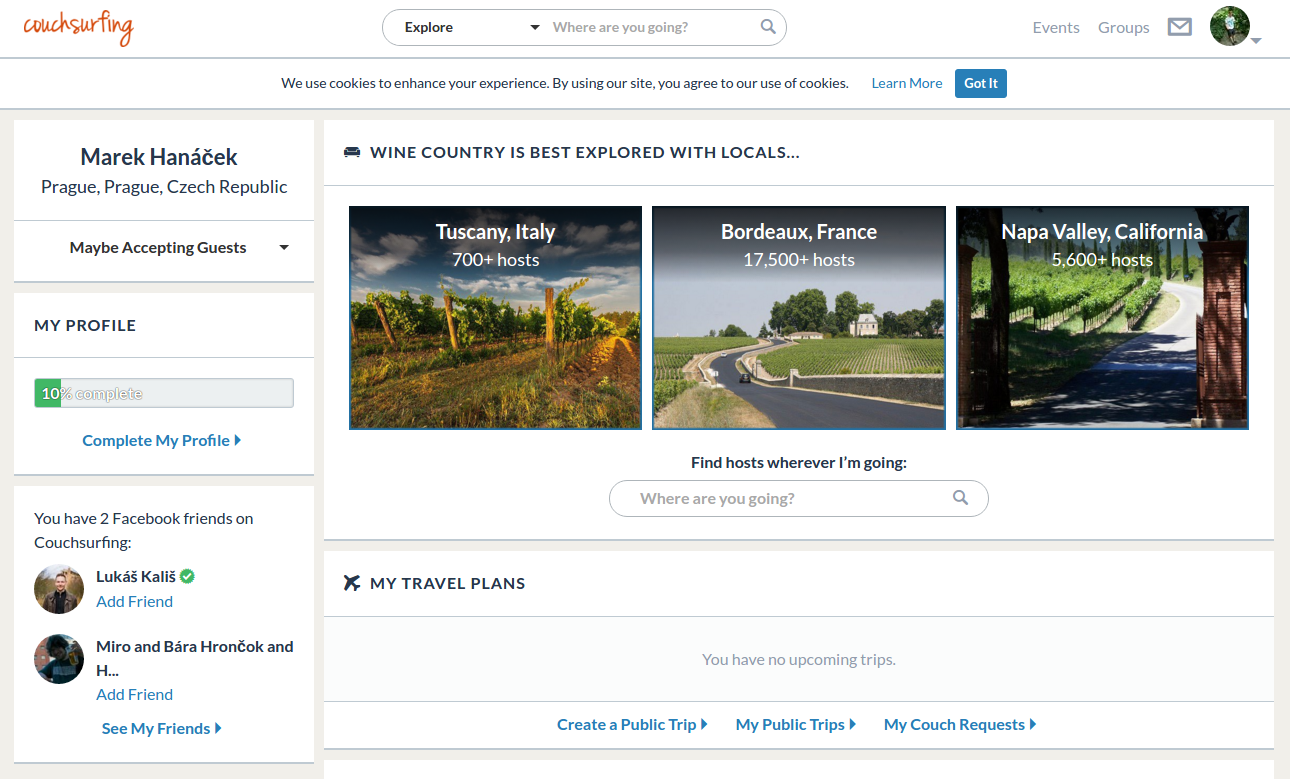
\includegraphics[width=1.0\textwidth]{media/couchsurfing/homepage.png}
    \caption{Couchsurfing.com -- Hlavní stránka}
    \label{fig:couchsurfing:homepage}
\end{figure}
\subsubsection*{Pozitiva}
\begin{itemize}
    \item[+] \textbf{Přehlednost} -- Všechno důležité na jednom místě a přehledně oddělené.
    \item[+] \textbf{Vyhledávací okno} -- Rychlé vyhledávací okno v~horní části stránky.
\end{itemize}
\subsubsection*{Negativa}
\begin{itemize}
    \item[-] \textbf{Stránka je dlouhá} -- Pro zobrazení veškerého obsahu je potřeba se dlouze posouvat po stránce.
\end{itemize}


%%%%%%%%%%%%%%%%%%%%%%%%%%%%%%%%%%%%%%%%%%%%%%%%%%%%%%%%%%%%%%%%%%%%%%%%%%%%%%%%%%%%%%%%%%%%%%%%%%%%%%%%%%%%%%%%%%%%%%%%

\newpage
\subsection{Vyhledávání ubytovaní}
Viz obrázek \ref{fig:couchsurfing:search}.
\begin{figure}[h]
    \centering
    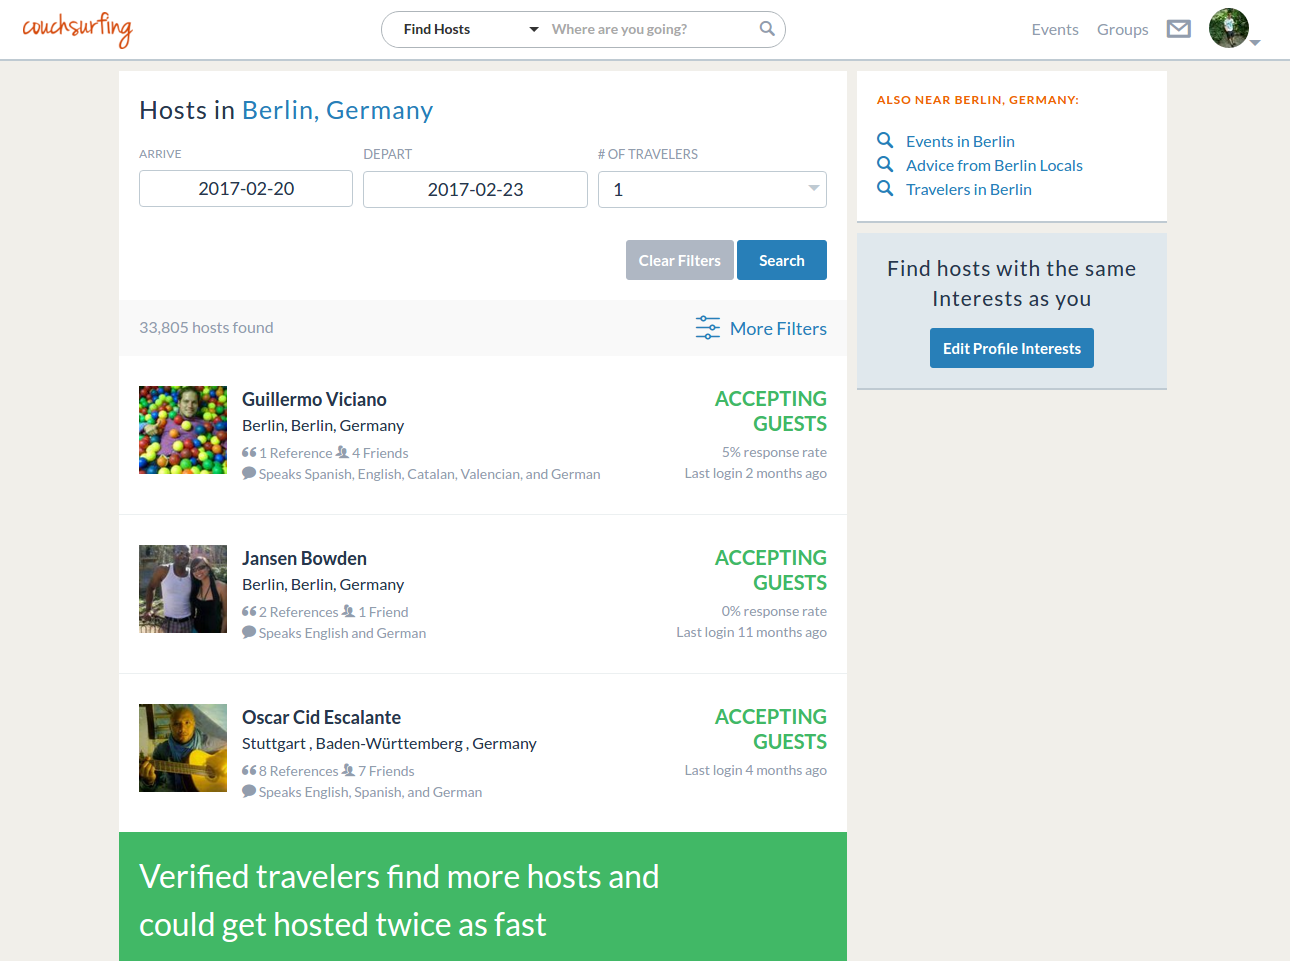
\includegraphics[width=1.0\textwidth]{media/couchsurfing/search.png}
    \caption{Couchsurfing.com -- Vyhledávání ubytování}
    \label{fig:couchsurfing:search}
\end{figure}
\subsubsection*{Pozitiva}
\begin{itemize}
    \item[+] \textbf{Jednoduchost}
    \item[+] \textbf{Filtry} -- Všechno důležité s~možností rozšířeného filtru.
    \item[+] \textbf{Status} -- Ověření uživatelé jsou jasně viditelní.
\end{itemize}
\subsubsection*{Negativa}
\begin{itemize}
    \item[-] \textbf{Žádná negativa na této stránce nejsou pozorována.}
\end{itemize}


%%%%%%%%%%%%%%%%%%%%%%%%%%%%%%%%%%%%%%%%%%%%%%%%%%%%%%%%%%%%%%%%%%%%%%%%%%%%%%%%%%%%%%%%%%%%%%%%%%%%%%%%%%%%%%%%%%%%%%%%

\newpage
\subsection{Profil uživatele}
Viz obrázek \ref{fig:couchsurfing:profile}.
\begin{figure}[h]
    \centering
    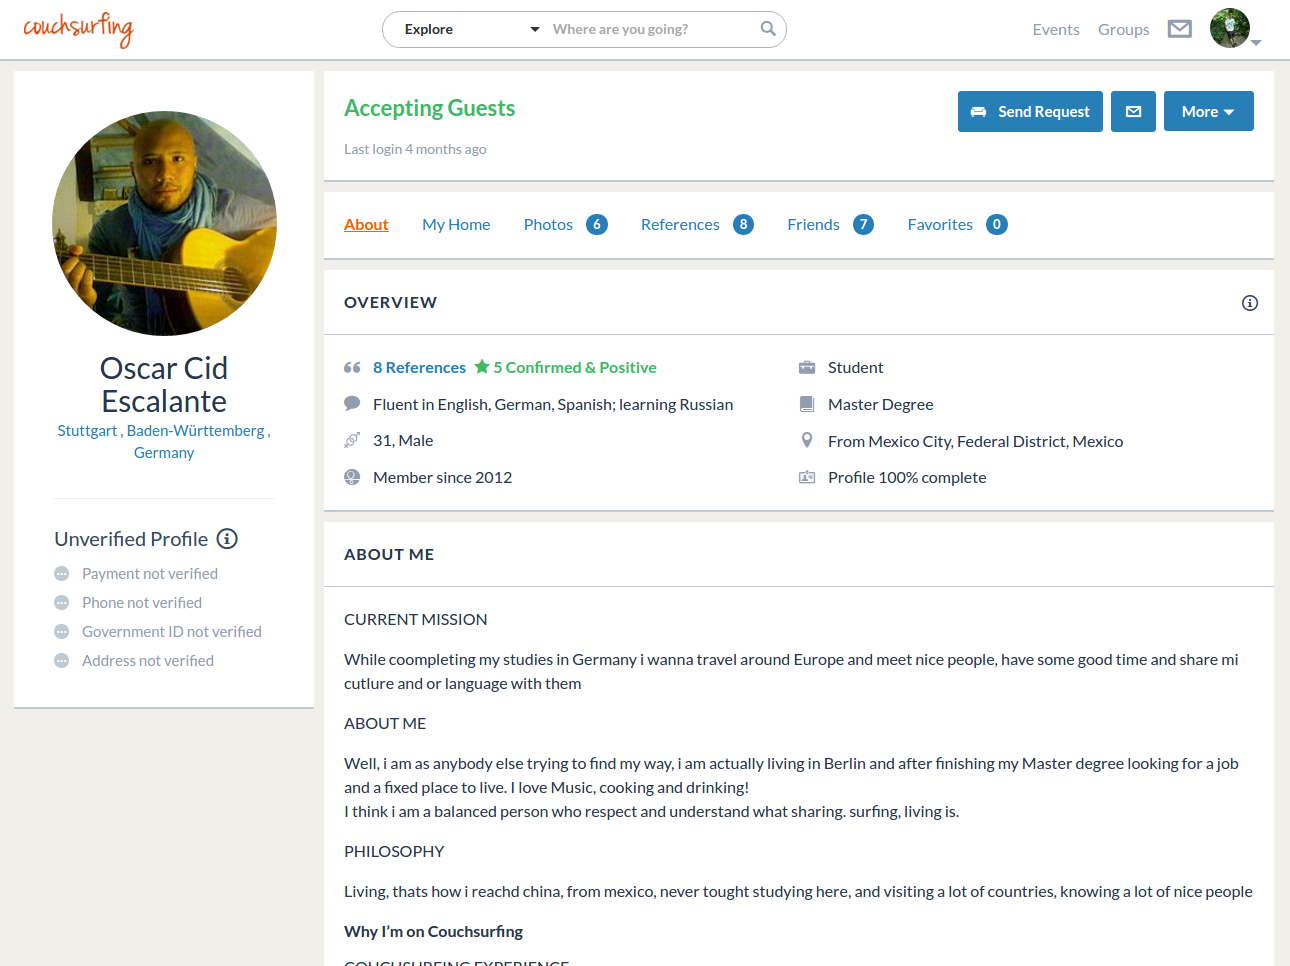
\includegraphics[width=1.0\textwidth]{media/couchsurfing/profile.png}
    \caption{Couchsurfing.com -- Profil uživatele}
    \label{fig:couchsurfing:profile}
\end{figure}
\subsubsection*{Pozitiva}
\begin{itemize}
    \item[+] \textbf{Informativnost} -- Všechno kompaktně na jednom místě a přehledně.
    \item[+] \textbf{O~uživateli} -- Popis uživatele uživatelem samotným. Jistě vítaná funkcionalita.
\end{itemize}
\subsubsection*{Negativa}
\begin{itemize}
    \item[-] \textbf{Žádná negativa na této stránce nejsou pozorována.}
\end{itemize}


%%%%%%%%%%%%%%%%%%%%%%%%%%%%%%%%%%%%%%%%%%%%%%%%%%%%%%%%%%%%%%%%%%%%%%%%%%%%%%%%%%%%%%%%%%%%%%%%%%%%%%%%%%%%%%%%%%%%%%%%

\newpage
\subsection{Shrnutí}
Celkově se webová aplikace Couchsurfing jeví velmi dobře řešená.

Důležitým mottem, se kterým je budována webová aplikace, je být \textbf{přehledný}. Každá podstránka by měla obsahovat vše co je potřeba a nic víc. Zajímavou myšlenkou je existence \textbf{verifikovaných uživatelů}, která by v~této práci vytvořila důvěru a určitou záruku korektního jednání při výměně peněz. Nevýhodu je velmi dlouhé provedení úvodní stránky, čehož je potřeba se vyvarovat a tím pádem ulehčit uživateli orientaci na stránce.